% ======================================================= %
% Document: TEMPLATE FOR RESPONSES TO REVIEWERS
% Author: Andrea Ballatore
% Date: Jan 7, 2013
% Source: https://raw.githubusercontent.com/ucd-spatial/Datasets/master/tex_response_to_reviewers_template/responses_to_reviewers.tex
% Modified by Eduard Szöcs, 10.03.2015
% ======================================================= %
\documentclass[12pt]{article}

% packages
\usepackage{xr}
\externaldocument[ms-]{Forecasting_revision1}

\usepackage{graphicx}
\usepackage{url}
\usepackage[usenames,dvipsnames]{xcolor}
\usepackage{color}
\definecolor{mygray}{gray}{0.6}
\usepackage[utf8]{inputenc}
\usepackage[onehalfspacing]{setspace}
\usepackage[
	round,	%(defaultage in the main file and \input ) for round parentheses;
	colon,	% (default) to separate multiple citations with colons;
	authoryear,% (default) for author-year citations;
	sort,		% orders multiple citations into the sequence in which they
]{natbib}
\usepackage[%disable
	]{todonotes}

\usepackage{anysize}
\graphicspath{{/Users/jm200/Library/CloudStorage/Dropbox/Miller Lab/github/POAR-Forecasting/Manuscript/Figures/}}
\marginsize{2.5cm}{2.5cm}{1.5cm}{2.5cm}

% macros
% add a counter
\newcounter{cN}
\setcounter{cN}{0}

\newcommand{\comment}[1]{
	\vspace{2em}
	\refstepcounter{cN} % incrment counter
	\noindent \hangindent=0em \textbf{\textcolor{Maroon}{\uline{Comment \thecN}:~}}\emph{``#1''}
	}

\newcommand{\response}[1]{
	\\[0.25em]
	\hangindent=2.3em \textbf{\textcolor{NavyBlue}{\uline{Response}:~}}#1
	}

\newcommand{\revise}[1]{{\color{Mahogany}{#1}}}

\usepackage[normalem]{ulem}
\definecolor{darkred}{rgb}{1,.6,.6}
\DeclareRobustCommand\problemline{\bgroup\markoverwith{\textcolor{darkred}{\rule[-0.9ex]{4pt}{3pt}}}\ULon}
\DeclareRobustCommand{\problem}[1]{\problemline{#1}} % soul
\setcounter{secnumdepth}{-1}

\begin{document}
% ======================================================= %
\title{Manuscript 2024-22162 --- Response to reviewers}

\maketitle
% ======================================================= %
\noindent To the editorial board,

Thank you for the opportunity to submit a revision of our manuscript for your consideration. Our major changes include the following:
\begin{enumerate}
	\item We have updated  Figure 3 as suggested by the reviewers.
	\item We increased the paper’s accessibility and impact for a broad PNAS audience by: 
	\begin{itemize}
	\item Including elements related to the effect of climate change on sex ratio in the discussion. 
	\item Discussing the potential mechanisms by which the dormant season affects population dynamics..
	\item Clarifying our methods and providing more precision regarding the modeling and statistics aspects of our work, including how we included the operational sex ratio (OSR), seed germination, seed variability in our model and the discrete matrix population model (MPM).
	\item Outlining the importance of both seasons  (dormant and growing season).
	\end{itemize}
\end{enumerate}

We describe these and other changes in greater detail below, where we reproduce comments from the associate editor and reviewers and provide our point-by-point responses. 
All of our changes are denoted in the manuscript with \revise{Mahogany font}.
We think the review process has greatly strengthened our manuscript such that it is now suitable for publication.
We hope you agree. 

\vspace{2em}
\hfill On behalf of myself , Tom Miller and A. Compagnoni,

\hfill  Jacob Moutouama
\newpage

% ======================================================= %
\section{Response to  the editor}
\vspace{-2em}

\comment{This study adds a novel element to our current knowledge of demographic impacts of climate change, by considering how operational sex ratios may be affected. Both reviewers appreciated the novelty, interest, and general soundness of the study. However, Rev. 1 raised some points about the statistics and modeling that need to be addressed, and Rev. 2 posed some excellent suggestions for increasing the paper's accessibility and impact for a broad PNAS audience. A revision should thoroughly respond to both sets of points.}
\response{We are grateful to  the editor for these  insightful comments on our manuscript. 
We agree with all these comments and have now addressed them in full in the revised manuscript, which is significantly improved as a result. 
More   specifically:
\begin{enumerate}
	\item We Clarified our methods and provided more precision regarding the modeling and statistics aspects of our work, including how we included the operational sex ratio (OSR), seed germination, seed variability in our model and the discrete matrix population model (MPM) as suggested by reviewer 1.
	\item We increased the paper’s accessibility and impact for a broad PNAS audience as suggested by reviewer 2.
\end{enumerate}
}

\section{Response to Reviewer 1}
\vspace{-2em}

\comment{
\\
Suitable Quality? Yes
\\
Sufficient General Interest? Yes
\\
Conclusions Justified? Yes
\\
Clearly Written? Yes
\\
Procedures Described? Yes
\\
Supplemental Material Warranted? Yes
\\
Sufficient data/samples? Yes.
}
\response{We thank Reviewer 1 for this  evaluation.}

\comment{Overall I thought this was a well written manuscript and a well conducted experiment and modeling exercise, tackling an interesting question. In particular, it is an interesting case study for why demographic approaches to species range questions may improve on occurrence or abundance based SDMs. The combination of sex-specific climate responses and feedback between sex ratio and reproductive success is not something that could be captured with a standard SDM, as far as I can imagine. Although there were some differences in predictions made with and without taking into account this feedback, I also appreciated the authors’ balanced treatment of the findings, discussing how the need to incorporate this biological nuance may depend on the questions of interest to researchers. For generalizing this result, a lot seems to hinge on the point they raise about needing to know the costs of reproduction for different sexes for more species. But this paper offers a
useful case study for how dioecious species may respond to changing climate.}
\response{We thank Reviewer 1 for these positive comments.}

\comment{ Overall the authors do a commendable (and appropriate) job of propagating uncertainty in their analyses. However, it was hard for me to tell whether that was also done for the parameters estimated in the previous sex ratio experiment, or if mean parameters were used? This seems quite important as that’s the key
relationship for distinguishing the two-sex model}
\response{We have propagated the uncertainty in the parameters estimated from the previous sex ratio experiment using Bayesian statistics. 
These details are now included in the main text (line 562- line 569) as well as in the supplementary material (line 46 and line 61).}

\comment{ Fig S13 shows how seed viability is related to OSR in that experiment, declining over ~ 75\% OSR, but also highlights
the very large apparent variability in that relationship. It was also unclear to me whether seed number was affected by OSR and was included in the model, or only
viability? It would be nice to include in this paper some discussion of why OSR affects seed viability, for those readers not familiar enough with plant reproductive
biology.}
\response{Both seed number and seed germination were included in the model, as they both influence population dynamics. 
We clarified this in the manuscript (line  516).
We appreciate the suggestion to include a discussion on why OSR affects seed viability.
We referenced our previous study\footnote{Compagnoni A, Steigman K, Miller TE (2017). Can’t live with them, can’t live without them? balancing mating and competition in two-sex populations. Proceedings of the Royal Society B: Biological Sciences 284(1865):20171999} that tested the effect of OSR on seed viability in the text and provided additional details in the supplementary material (line 53 - line 66).}

\comment{ I might have thought OSR would primarily affect seed number rather than viability. Do unfertilized ovules produce non-viable seeds in this species (they’re not simply aborted)?}
\response{We did not test whether OSR would primarily affect seed number. 
%However, in a previous study, we assessed OSR  effect on seed viability (Compagnoni et al. 2017). 
%We referenced our previous study\footnote{Compagnoni A, Steigman K, Miller TE (2017). Can’t live with them, can’t live without them? balancing mating and competition in two-sex populations. Proceedings of the Royal Society B: Biological Sciences 284(1865):20171999} that tested the effect of OSR on seed viability in the text (line 547 - line 551) and provided additional details in the supplementary material (line 53 - line 66)}.
%%The purpose of including  seed viability was to generate more realistic predictions for the demographic model.
%\\
%\\
Yes, in \emph{Poa arachnifera}, unfertilized ovules can lead to the production of non-viable seeds. This phenomenon is part of a reproductive strategy called apomixis, where seeds can develop without fertilization. In this case, the seeds produced from unfertilized ovules typically do not contain viable embryos and, therefore, do not germinate.}

\comment{It seems important to have some discussion of the potential mechanism by which dormant season climate could be important, and how these predictions are
different than for growing season climate.}
\response{We agree with the reviewer on this.  
We added a discussion of the potential mechanism by which dormant season climate could be important, in the discussion where we stated (line  354- line 368): “\emph{Climate conditions during the dormant season are at least as important as those during the growing season. 
This result contrasts with a recent synthesis suggesting that only the dormant season matters for plants. 
Temperature and precipitation during the dormant season significantly impact population dynamics. 
For instance, the reduction of snowpack, which protects plants from frost damage through insulation, could decrease plants probability of flowering. 
Similarly, a reduction in snowfall could diminish water storage in the soil, negatively affecting plant survival and growth".}}

\comment{Why does precip have a negative effect on most vital rates in this seasonally arid region?.}
\response{Good question.
We answered that question in the discussion where we stated (line 363 - line 368): “\emph{Intense precipitation may lead to flooding or waterlogged soils, which can harm plant roots and consequently reduce their growth and survival. 
Furthermore, increase precipitation  could stimulate rapid plant growth, leading to increased competition for resources among species}”.
}

\comment{ Since there are mixed models of the vital rates, as a continuous function of size, I didn’t follow why discrete MPM were used instead of IPMs. I assume there’s a good reason, given the authors’ expertise, but not clear why discrete model used and how all the individual transitions were estimated. Maybe the mixed models were discretized, like an IPM ends up doing in practice, and I just didn’t understand? It’s hard to imagine how climate effects on that many discrete transitions would be estimated.}
\response{}

\comment{ And U is 35 tillers; how many size stages do the models have?}
\response{The model has 35 stages. We clarified that in the manuscript (line 528- line 530.}

\comment{Fig S3 – says 95\% CI but two intervals shown}
\response{Thank you. We want to ensure we address the  concerns of Reviewer 1 accurately, but we  having some difficulty understanding  his question. 
Where are the two intervals in the Figure S3 ?}

\comment{L104 says most sex coefficients were significant, but this isn’t obvious from Fig S3 (most seem overlapping zero); perhaps authors could be more specific about which rates they conclude are significant, or include probabilities of overlap with zero.}
\response{Thank you for  this comment.
We have softened the language and added more specificity regarding vital rates (line 106).}

\comment{Text says 8 source pops. In Fig 1 I only count 7?}
\response{We thank the reviewer for this suggestion. 
We have updated the number of source populations to seven in the text (line 462).}

\comment{Fig 2 – maybe show shaded uncertainty regions on the regression?}
\response{We appreciate the suggestion. However, adding shaded uncertainty regions to the regression would be misleading for several reasons:
\begin{itemize}
\item The 95\% uncertainty shading would make the plot cluttered and fail to accurately represent our findings. 
Please see the plot below.
While the vital rates account for differences in sites and source populations, they do not capture the three-way interaction, as the plot is presented in two dimensions. 
This is why we included a 3D plot in the supplementary material (Fig S4 and Fig  S5).
\item However, if the associate editor and the reviewer would like us to include this in the manuscript, we can certainly do so.
We have propagated the uncertainty (from both site and population differences, as well as parameters) from the vital rates to the probability of lambda being greater than 1. 
\end{itemize}

\begin{figure}[h]
\centering
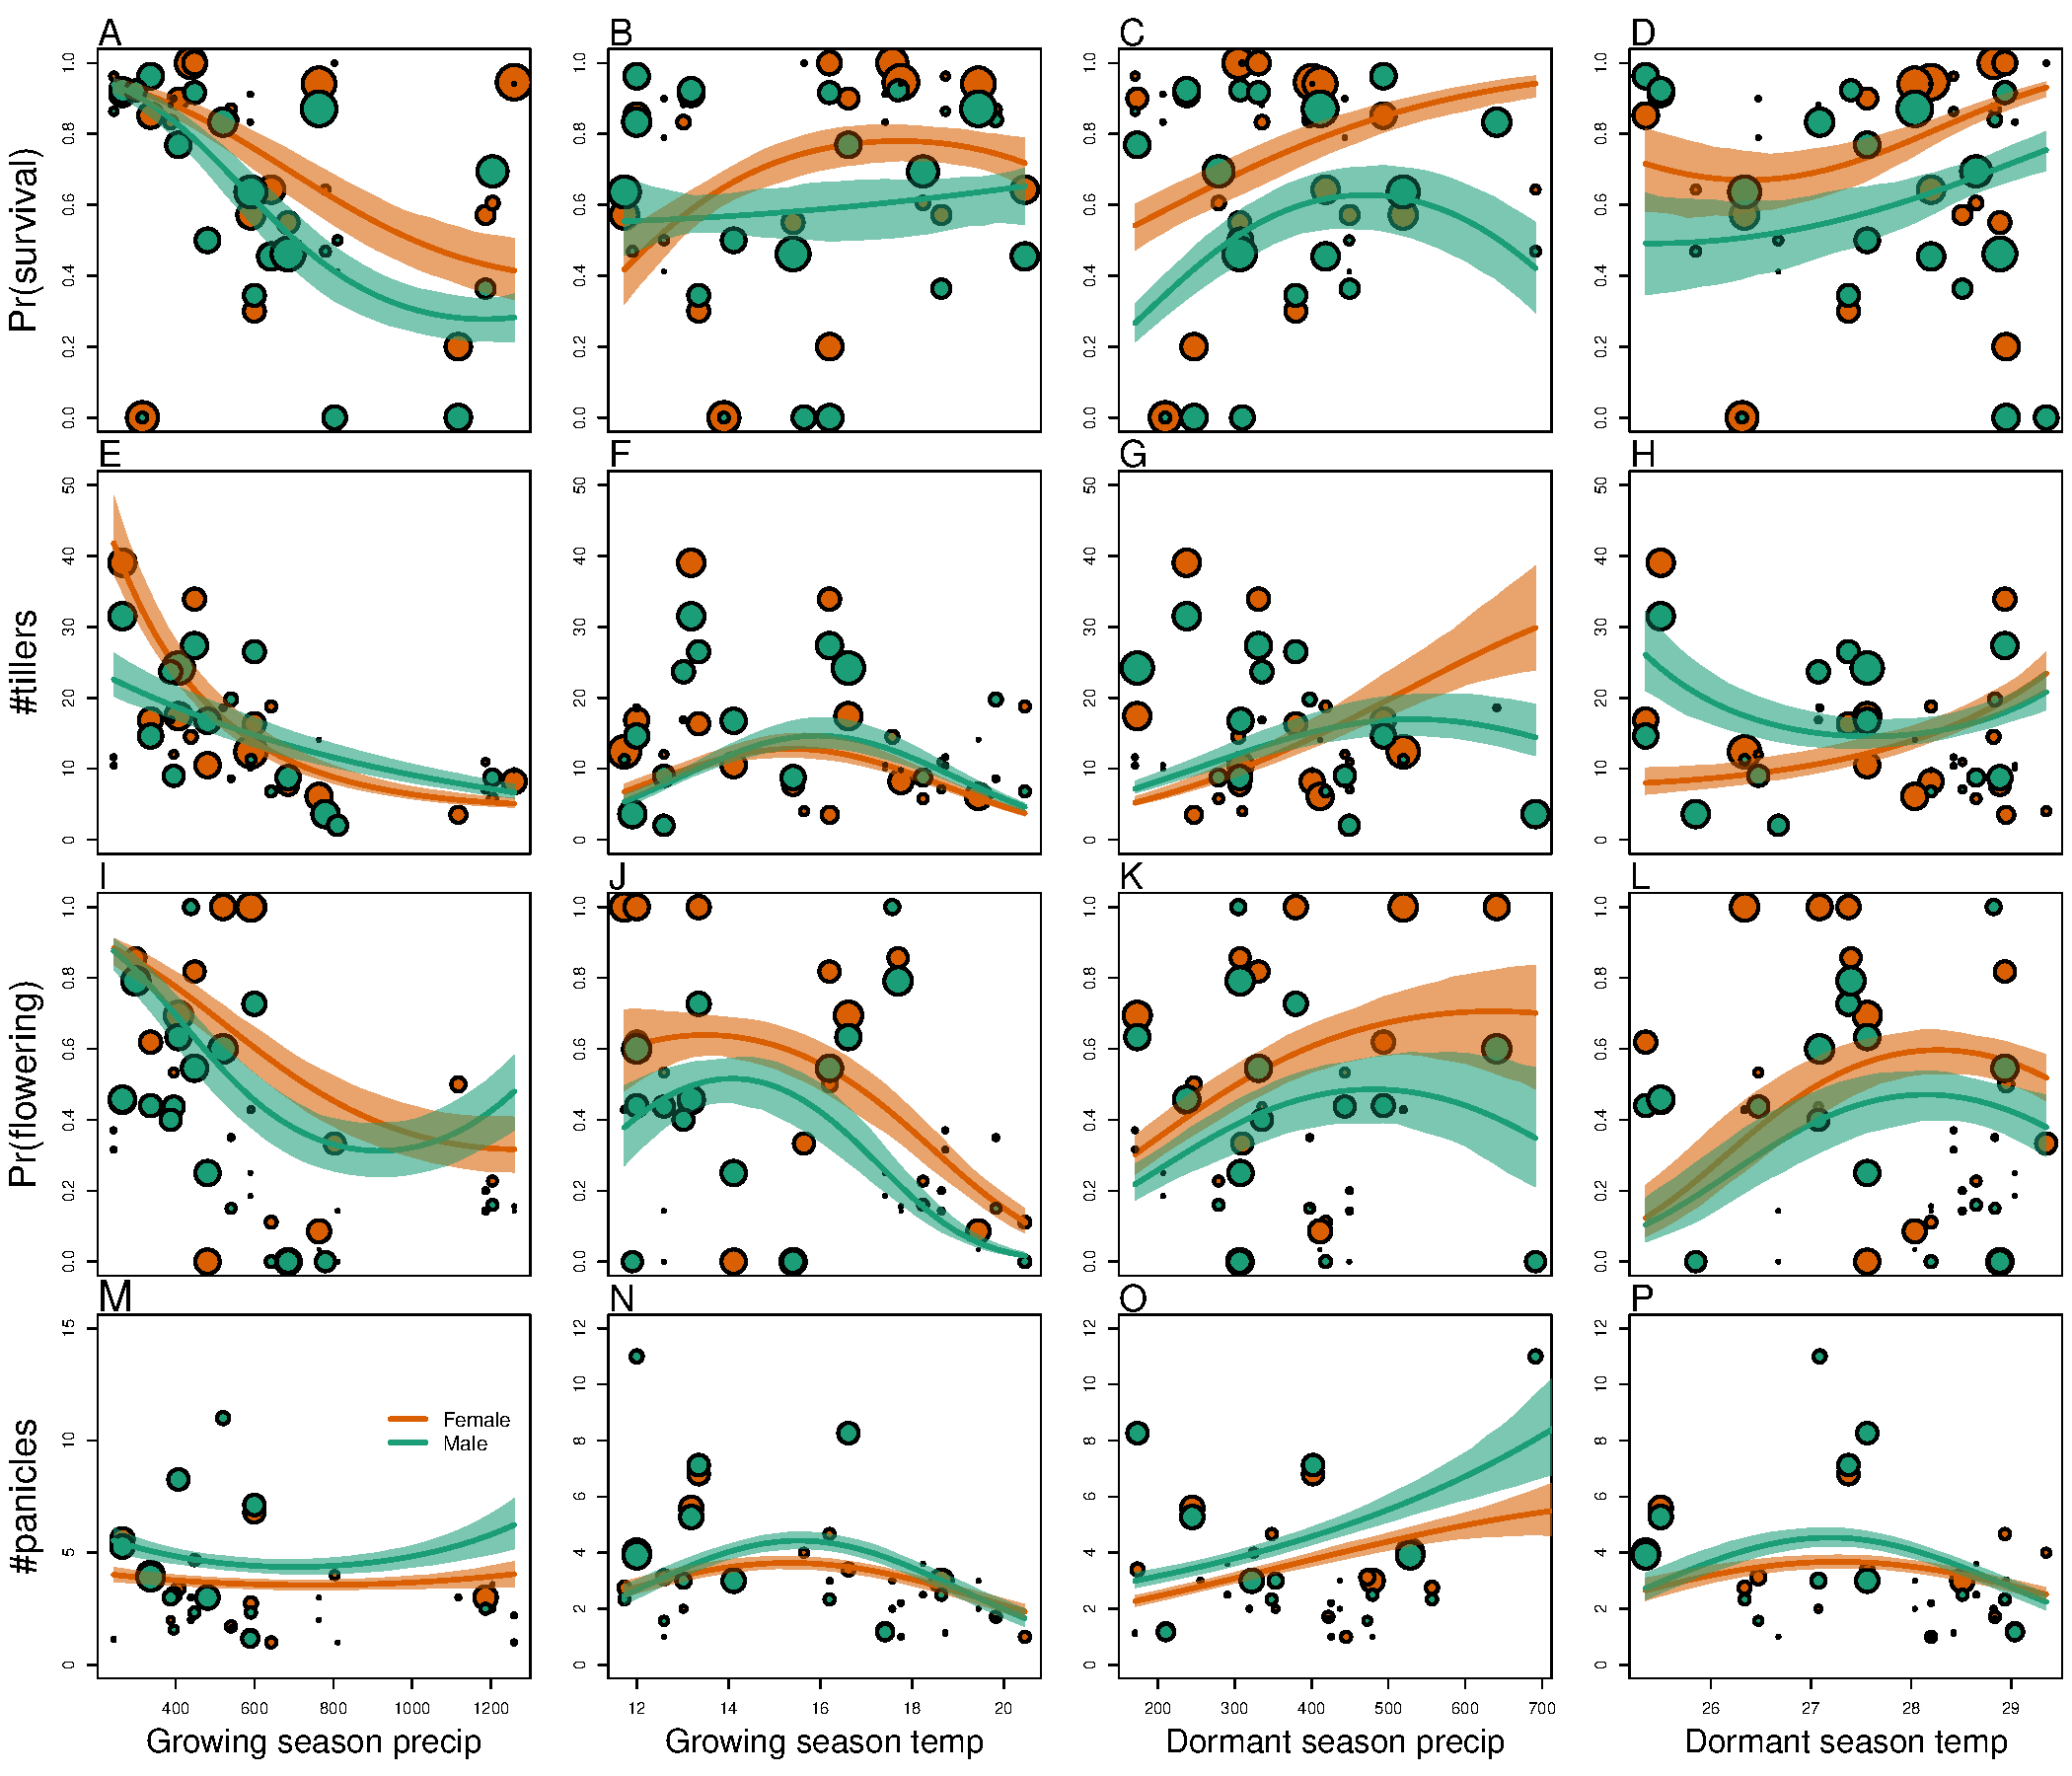
\includegraphics[width=1\linewidth]{vital_rates_v1_r1.pdf}
\label{fig:vital_rates}
\end{figure}
}

\comment{L176, 179 – are these referring to the wrong figure panels? E and F show the difs between the sex and no-sex models I believe}
\response{Yes these were referring to the wrong figure panels. We  have updated  the Figure panels (line 176).}

\comment{ Fig 3 – the plot of past, current and future points is hard to eyeball any patterns. Maybe in addition a histogram or density plot of the values to show any shifts in probabilities?}
\response{ We appreciate this suggestion. 
We have updated Figure 3 by removing the observed climate values and replacing the last two panels with density plots to illustrate any shifts in probabilities, as  recommended.}

\section{Response to Reviewer 2}
\vspace{-2em}

\comment{
\\
Suitable Quality? Yes
\\
Sufficient General Interest? Yes
\\
Conclusions Justified? Yes
\\
Clearly Written? No
\\
Procedures Described? Yes
\\
Supplemental Material Warranted? Yes
\\
Sufficient data/samples? Yes.
}
\response{We thank  reviewer 2 for   this evaluation.}


\comment{It is accurate and well written, but describes the advances in a way that would appeal to a specialized audience of ecologists, rather than a general audience. See my comments along these lines in the main manuscript review}
\response{We appreciate this reviewer's supportive comments and constructive suggestions.}

\comment{This is a great paper, addressing the projected impacts of climate change on plant species distributions. Within the field of demography, it is a substantial advance empirically because it is based on demographic studies done throughout a species current range and because it shows that a substantial contribution to the species' range shift comes from changes in sex ratio of this dioecious plant species. Understanding the contribution of sex ratio to plant population growth rates required novel aspects of the experimental field design and of the population projection models. In my opinion this study is one of the very best in the field, and could be well-placed in PNAS.}
\response{We  appreciate  the reviewer for these comments.}

\comment{However, the study as currently written strikes me as being written for other plant ecologists and demographers - an Ecology or Journal of Ecology audience, not a PNAS audience. I am a plant demographer, so I would defer to others outside the field if they read the manuscript and see the exciting results as written. But, in the event that other reviewers do not see the substantial advance made by this paper, I believe the manuscript could be made exciting to a general audience by emphasizing the following points:
\\
1. Climate change is changing the operational sex ratio of plant populations. This change is not due to something direct like temperature-dependent sex determination, but to climate-induced changes in vital rates later in life. Many organisms are likely to have sex-dependent vital rates, and interactions of climate with these differences. Changes in sex ratio are an under-appreciated (and kind of creepy) implication of climate change that could appeal broadly to the general public. This point could, for example, get at least one paragraph in the discussion, in relation to other studies that have shown effects of climate change on sex ratio, in both animals and plants.}
\response{ We thank the reviewer for this comment. We have now elaborated on how climate change could affect the operational sex ratio of plant populations.(line 332 - line 353).}

\comment{2. Climate conditions during the non-growing season were at least as important as climate conditions during the growing season. These results are currently in an appendix, but I suggest moving them to the main text. Off the top of my head, I am not aware of many (any?) other plant demogrpahy studies that have addressed this question explicitly. To a broad group of readers (scientists and the general public), I think it could be amazing that times when organisms are dormant matter as much as times of the year when they are active. How often has this been done in other studies? How much do we know about seasonality in projected impacts of climate change?}
\response{In the text, we mentioned that climate conditions during the non-growing season are at least as important as those during the growing season. We stated, \emph{'These visual trends are supported by Life Table Response Experiment (LTRE) decomposition, indicating that variation in fitness across climatic conditions is most strongly driven by responses to growing and dormant season temperatures, with weaker interactive effects of precipitation that modulate the effects of temperature (Fig. S9)'} (line 146 - line 156). Unfortunately, we cannot move a figure from the Appendix to the main text, as the maximum number of figures is limited to four. That said, we have added a discussion paragraph on the impact of seasonality on population dynamics (line 354 - line 358).}

\comment{3. The result that the two models make broadly similar predictions is important and comforting. As written, the paper emphasizes the differences between projections from models that account for sex-ratio and from traditional female-only demographic models. I would give at least as much time to the similarities. Qualitatively, we are getting the right patterns with conventional methods, and, although the devil is in the details of the biology, there are also a lot of details of the climate, habitat, potential for local adaptation, etc that are missing. This result is good news in the sense that not all details fundamentally change the story of climate change impacts. (Even though the simple models miss the creepy and cool changes in sex ratio for this species.)}
\response{Thank you for this valuable suggestion.
 The paper highlights both the differences and similarities between projections from models that account for sex ratios and traditional female-only demographic models. 
 For instance, we discuss these similarities in the discussion section, where we state: \emph{"Predictions of the two-sex and female-dominant models were in strong agreement about climate niche optima, and LTRE decomposition suggested that female vital rates determine population responses to climate variation much more so than male vital rates. 
If we wanted to know whether a poleward range shift is likely for Texas bluegrass, the simpler female-dominant approach could have given us the correct answer. 
This is good news from a conservation standpoint because most studies on dioecious species rely on models that assume male availability has no influence on female fertility.
} " (line 273 - line 303). 
 Additionally, we address this topic in the conclusion, noting:\emph{ "But in broad strokes, a female-dominant perspective tells much of the story, and that will likely be true for dioecious plants and animals with mating systems in which few males can fertilize many females.} " (line 398 - line 401)
Furthermore, we have now elaborated on the implications of these similarities for conservation actions related to dioecious species in the discussion section (line 413 - line 416.}

\comment{As a minor comment, I suspect Figure 3 would be especially hard for a nonspecialist to understand, and I encourage the authors to think about a simpler message they might want to convey in a different figure in the main text. (Again, I say this as a specialist trying to imagine myself as a nonspecialist reading the paper.)}
\response{We appreciate this suggestion. 
We have updated Figure 3 by removing the observed climate values and replacing the last two panels with density plots to illustrate any shifts in probabilities, as  recommended.}


% ======================================================= %
\end{document}
% ======================================================= %
